\documentclass[12pt,a4paper,UTF8]{ctexart} % 使用 ctexart，内置中文支持

% --- 核心宏包设置 ---
\usepackage{geometry}      % 页边距设置
\usepackage{amsmath}       % 数学公式
\usepackage{enumitem}      % 列表格式控制
\usepackage{graphicx}      % 插入图片
\usepackage{hyperref}      % 超链接
\usepackage{setspace}      % 行间距控制
\usepackage{titlesec}      % 标题格式定制
\usepackage{booktabs}      % 专业表格线
\usepackage{listings}      % 用于插入代码
\usepackage{xcolor}        % 代码高亮配色
\usepackage{subfig}        % 用于并排对比图
\usepackage{tcolorbox}     % 【新增】用于创建精美的对比框
\usepackage{fancyhdr}      % 【新增】用于设置页眉页脚
\tcbuselibrary{skins,breakable}

% --- 页面与格式设置 ---
% --- 页眉页脚设置 ---
\pagestyle{fancy}
\fancyhf{}
\fancyhead[L]{\small \itshape 基于灰度世界算法的自动白平衡校正}
\fancyhead[R]{\small \thepage}
\renewcommand{\headrulewidth}{0.4pt}

% --- 自定义对比框样式 ---
\newtcolorbox{mycompare}[1]{
    colback=blue!5!white,
    colframe=blue!75!black,
    fonttitle=\bfseries,
    title=#1,
    enhanced,
    attach boxed title to top left={xshift=3mm, yshift=-3mm, yshifttext=-1mm},
    boxed title style={colback=blue!75!black},
    sharp corners,
    drop shadow
}

\newtcolorbox{myresult}[1]{
    colback=green!5!white,
    colframe=green!50!black,
    fonttitle=\bfseries,
    title=#1,
    enhanced,
    attach boxed title to top left={xshift=3mm, yshift=-3mm, yshifttext=-1mm},
    boxed title style={colback=green!50!black},
    drop lifted shadow
}

% --- 代码高亮全局设置 ---
\lstset{
    language=Python,
    basicstyle=\ttfamily\small,
    keywordstyle=\color{blue!80!black}\bfseries,
    commentstyle=\color{gray!70!black}\itshape,
    stringstyle=\color{orange!90!black},
    numbers=left,
    numberstyle=\tiny\color{gray},
    frame=single,
    frameround=tttt,
    bordercolor=\color{gray!20},
    breaklines=true,
    captionpos=b,
    escapeinside=``,
    xleftmargin=2em,
    xrightmargin=2em,
    aboveskip=1.5em,
    belowskip=1.5em,
    backgroundcolor=\color{gray!5}
}

% --- 文档开始 ---
\begin{document}

% ======================================================
% 1. 独立封面页
% ======================================================
\begin{titlepage}
    \centering
    \vspace*{3cm}
    
    % 主标题
    {\Huge \bfseries 基于灰度世界算法的照片自动白平衡校正工具 \par}
    \vspace{1.5cm}
    % 副标题
    {\Large \textbf{技术调研与方案实现研究报告} \par}
    
    \vspace{4.5cm}
    
    % 个人信息表格：优化了对齐和边距
    \begin{minipage}{0.6\textwidth}
        \centering
        \large
        \renewcommand{\arraystretch}{1.6} 
        \begin{tabular}{r l}
            \textbf{姓名：} & 王为韬 \\
            \textbf{学院：} & 武汉大学人工智能学院 \\
            \textbf{日期：} & 2026年2月26日 \\
        \end{tabular}
    \end{minipage}

    \vfill

    % 底部校名
    {\Large \textbf{武汉大学} \par}
    {\large Wuhan University \par}
    \vspace{1cm}
    
\end{titlepage}

% ======================================================
% 2. 目录页
% ======================================================
\newpage
\tableofcontents
\newpage

% ======================================================
% 3. 正文内容
% ======================================================

\section{项目背景与研究意义}

在计算机视觉与图像处理领域，还原物体的真实色彩是后续一切分析任务的基础。由于拍摄环境的光源色温不同（如日落、荧光灯、阴天），图像往往会产生偏色现象。

本项目旨在通过研究 \textbf{自动白平衡（Auto White Balance, AWB）} 技术，对 ISP 过程中的数字信号进行校正。这不仅是理解数字成像链路的关键环节，也为后续水利监测、无人机航拍等复杂场景下的图像标准化提供了核心支持。

\section{数字成像链路与 ISP 流程分析}

理解白平衡的前提是掌握数字成像的完整生命周期。光线经过传感器转换后，需经过一系列算法处理才能生成人眼可见的图像：

\begin{center}
\fbox{真实世界光线} $\rightarrow$ 镜头 $\rightarrow$ 滤色镜 (Bayer Array) $\rightarrow$ 传感器 $\rightarrow$ ADC $\rightarrow$ \textbf{ISP (AWB/降噪/锐化)} $\rightarrow$ 压缩编码 $\rightarrow$ \fbox{最终照片}
\end{center}

白平衡处理发生在 ISP 阶段。其本质是通过统计学或物理模型，计算出 RGB 三通道的增益系数因子，从而补偿光源对物体反射光谱造成的偏移。

\section{技术路线：自动白平衡算法选型}

本项目对比了“曝光补偿”与“自动白平衡”两种方案，最终确定以 AWB 作为核心算法实践路径。

\begin{mycompare}{方案对比：曝光补偿 vs. 自动白平衡}
    \begin{itemize}
        \item \textbf{曝光补偿}：侧重于亮度的整体提升或降低，无法解决由于光源色温引起的“偏色”问题。
        \item \textbf{自动白平衡 (AWB)}：通过调整 RGB 三通道的比例，还原物体在标准白光下的真实色彩，是解决偏色的核心技术。
    \end{itemize}
\end{mycompare}

\subsection{算法选型综述}
\begin{itemize}
    \item \textbf{算法复杂度}：灰度世界算法涉及像素遍历与均值计算，数学推导清晰，适合工程落地。
    \item \textbf{视觉反馈}：AWB 对偏色图像的修复具有极强的视觉冲击力，能显著提升成片质量。
    \item \textbf{能力培养}：通过实现该算法，可以深度掌握通道分离、图像归一化等底层编程技能。
\end{itemize}

\section{核心算法原理：灰度世界模型}

本项目首选实现的算法模型为 \textbf{灰度世界算法 (Gray World Algorithm)}。其基本假设是：对于一幅有着大量色彩变化的图像，其 RGB 三个通道的平均值趋于同一个灰度值 $K$。

\subsection{原版灰度世界算法}
计算过程如下：
\begin{enumerate}
    \item 计算图像 R、G、B 三通道的平均反射强度：
    \[
    R_{avg} = \frac{1}{M \times N} \sum_{i=1}^{M} \sum_{j=1}^{N} R(i,j), \quad 
    G_{avg} = \frac{1}{M \times N} \sum_{i=1}^{M} \sum_{j=1}^{N} G(i,j), \quad 
    B_{avg} = \frac{1}{M \times N} \sum_{i=1}^{M} \sum_{j=1}^{N} B(i,j)
    \]
    其中 $M$ 为图像行数，$N$ 为图像列数，$R(i,j)$、$G(i,j)$、$B(i,j)$ 分别为第 $i$ 行第 $j$ 列像素的 R、G、B 通道值。
    
    本项目处理的是颜色插补后的全彩图像，每个像素包含完整 RGB 三通道信息，因此采用总像素数 M×N 计算通道平均值
    
    \item 设定全局参考灰度值：
    \[
    K = \frac{R_{avg} + G_{avg} + B_{avg}}{3}
    \]
    
    \item 计算各通道增益系数：
    \[
    k_r = \frac{K}{R_{avg} + 10^{-6}}, \quad 
    k_g = \frac{K}{G_{avg} + 10^{-6}}, \quad 
    k_b = \frac{K}{B_{avg} + 10^{-6}}
    \]
    式中 $10^{-6}$ 为防除零项，避免通道平均值为0时的计算错误。
    
    \item 利用增益系数对全图像素进行线性映射：
    \[
    R_{new}(i,j) = \min\left( \max\left( k_r \cdot R(i,j), 0 \right), 255 \right)
    \]
    \[
    G_{new}(i,j) = \min\left( \max\left( k_g \cdot G(i,j), 0 \right), 255 \right)
    \]
    \[
    B_{new}(i,j) = \min\left( \max\left( k_b \cdot B(i,j), 0 \right), 255 \right)
    \]
    通过 $\min$ 和 $\max$ 函数对映射后的像素值做截断处理，强制限定在 $[0,255]$ 范围，避免色彩失真。
\end{enumerate}

\subsection{优化版灰度世界算法}
原版算法使用全图像素计算通道均值，高光（亮度>180）或阴影（亮度<60）区域会严重干扰均值计算，导致校正偏差。优化版算法通过“中亮度像素筛选”解决该问题，核心改进如下：

\subsubsection{核心改进思路}
仅选取亮度在 $[60, 180]$ 区间的像素计算通道均值（该区间为图像的“有效纹理区域”，排除纯黑/纯白无信息像素），并增加“有效像素占比校验”：若中亮度像素占比<10%，自动切回原版算法，保证鲁棒性。

\subsubsection{数学推导}
\begin{enumerate}
    \item 将图像转换为灰度空间，筛选中亮度像素掩码：
    \[
    \text{Gray}(i,j) = 0.299 \cdot R(i,j) + 0.587 \cdot G(i,j) + 0.114 \cdot B(i,j)
    \]
    \[
    \text{mask}(i,j) = 
    \begin{cases}
    1, & 60 \leq \text{Gray}(i,j) \leq 180 \\
    0, & \text{其他}
    \end{cases}
    \]
    
    \item 计算有效像素占比：
    \[
    \rho = \frac{\sum_{i=1}^{M}\sum_{j=1}^{N} \text{mask}(i,j)}{M \times N}
    \]
    
    \item 分分支计算通道均值：
    \[
    R_{avg} = 
    \begin{cases}
    \frac{1}{\sum \text{mask}} \sum_{i=1}^{M}\sum_{j=1}^{N} R(i,j) \cdot \text{mask}(i,j), & \rho \geq 0.1 \\
    \frac{1}{M \times N} \sum_{i=1}^{M}\sum_{j=1}^{N} R(i,j), & \rho < 0.1
    \end{cases}
    \]
    $G_{avg}$、$B_{avg}$ 计算逻辑与 $R_{avg}$ 一致。
    
    \item 后续增益系数计算、像素映射与原版算法完全一致。
\end{enumerate}

\subsubsection{优化版核心代码实现}
\begin{lstlisting}[caption={优化版灰度世界算法核心实现}, label=code:awb_opt]
def gray_world_awb(image_path, use_optimized=True):
    img = cv2.imdecode(np.fromfile(image_path, dtype=np.uint8), cv2.IMREAD_COLOR)
    b, g, r = cv2.split(img)
    
    if use_optimized:
        # 转换为灰度图，筛选中亮度像素
        gray = cv2.cvtColor(img, cv2.COLOR_BGR2GRAY)
        mask = (gray >= 60) & (gray <= 180)
        valid_ratio = np.sum(mask)/mask.size
        
        # 有效像素占比≥10%才用优化版，否则切回原版
        if valid_ratio >= 0.1:
            b_avg = np.mean(b[mask])
            g_avg = np.mean(g[mask])
            r_avg = np.mean(r[mask])
        else:
            b_avg = np.mean(b)
            g_avg = np.mean(g)
            r_avg = np.mean(r)
    else:
        # 原版算法：全局均值
        b_avg = np.mean(b)
        g_avg = np.mean(g)
        r_avg = np.mean(r)
    
    # 后续增益计算与原版一致
    K = (b_avg + g_avg + r_avg) / 3.0
    gain_b = K / (b_avg + 1e-6)
    gain_g = K / (g_avg + 1e-6)
    gain_r = K / (r_avg + 1e-6)
    
    b_new = np.clip(b.astype(float) * gain_b, 0, 255)
    g_new = np.clip(g.astype(float) * gain_g, 0, 255)
    r_new = np.clip(r.astype(float) * gain_r, 0, 255)
    return cv2.merge([b_new.astype(np.uint8), g_new.astype(np.uint8), r_new.astype(np.uint8)])
\end{lstlisting}

\section{实验验证与结果分析}

为验证灰度世界算法的有效性与局限性，本项目使用 Python + OpenCV 实现了完整 Demo，选取6组典型场景进行测试，对比原版（v0）与优化版（v2）的校正效果，验证优化策略的有效性与算法边界。

\subsection{测试集与评价维度}
本次测试选取6组典型场景，分为三大类：
\begin{itemize}
    \item \textbf{极端低有效像素场景}：逆光人像、夜景路灯，验证优化版的自适应降级能力；
    \item \textbf{大面积纯色场景}：红色幕布，验证算法的固有局限性；
    \item \textbf{常规色彩丰富场景}：城市街道、怀旧小街、色彩鲜艳美食图，验证优化版的常规场景表现。
\end{itemize}
评价维度包括：色彩还原度、算法鲁棒性、画面氛围感保留度、校正偏差程度。

\subsection{场景一：优化版自适应降级能力验证}
针对逆光人像、夜景路灯这类“中亮度有效像素占比<10%”的极端场景，优化版算法会自动触发降级逻辑，切换为原版算法，避免有效信息不足导致的过度校正，保证算法鲁棒性。

\begin{table}[htbp]
    \centering
    \caption{极端场景算法行为与效果对比}
    \label{tab:adaptive_downgrade}
    \begin{tabular}{@{}cccc@{}}
        \toprule
        测试场景 & 中亮度像素占比 & 优化版算法行为 & 校正效果对比 \\
        \midrule
        逆光人像 & 4.2\% & 自动降级为v0 & 与原版效果完全一致，无额外失真 \\
        夜景路灯 & 2.7\% & 自动降级为v0 & 与原版效果完全一致，无额外失真 \\
        \bottomrule
    \end{tabular}
\end{table}

\begin{figure}[htbp]
    \centering
    \begin{minipage}{0.48\textwidth}
        \centering
        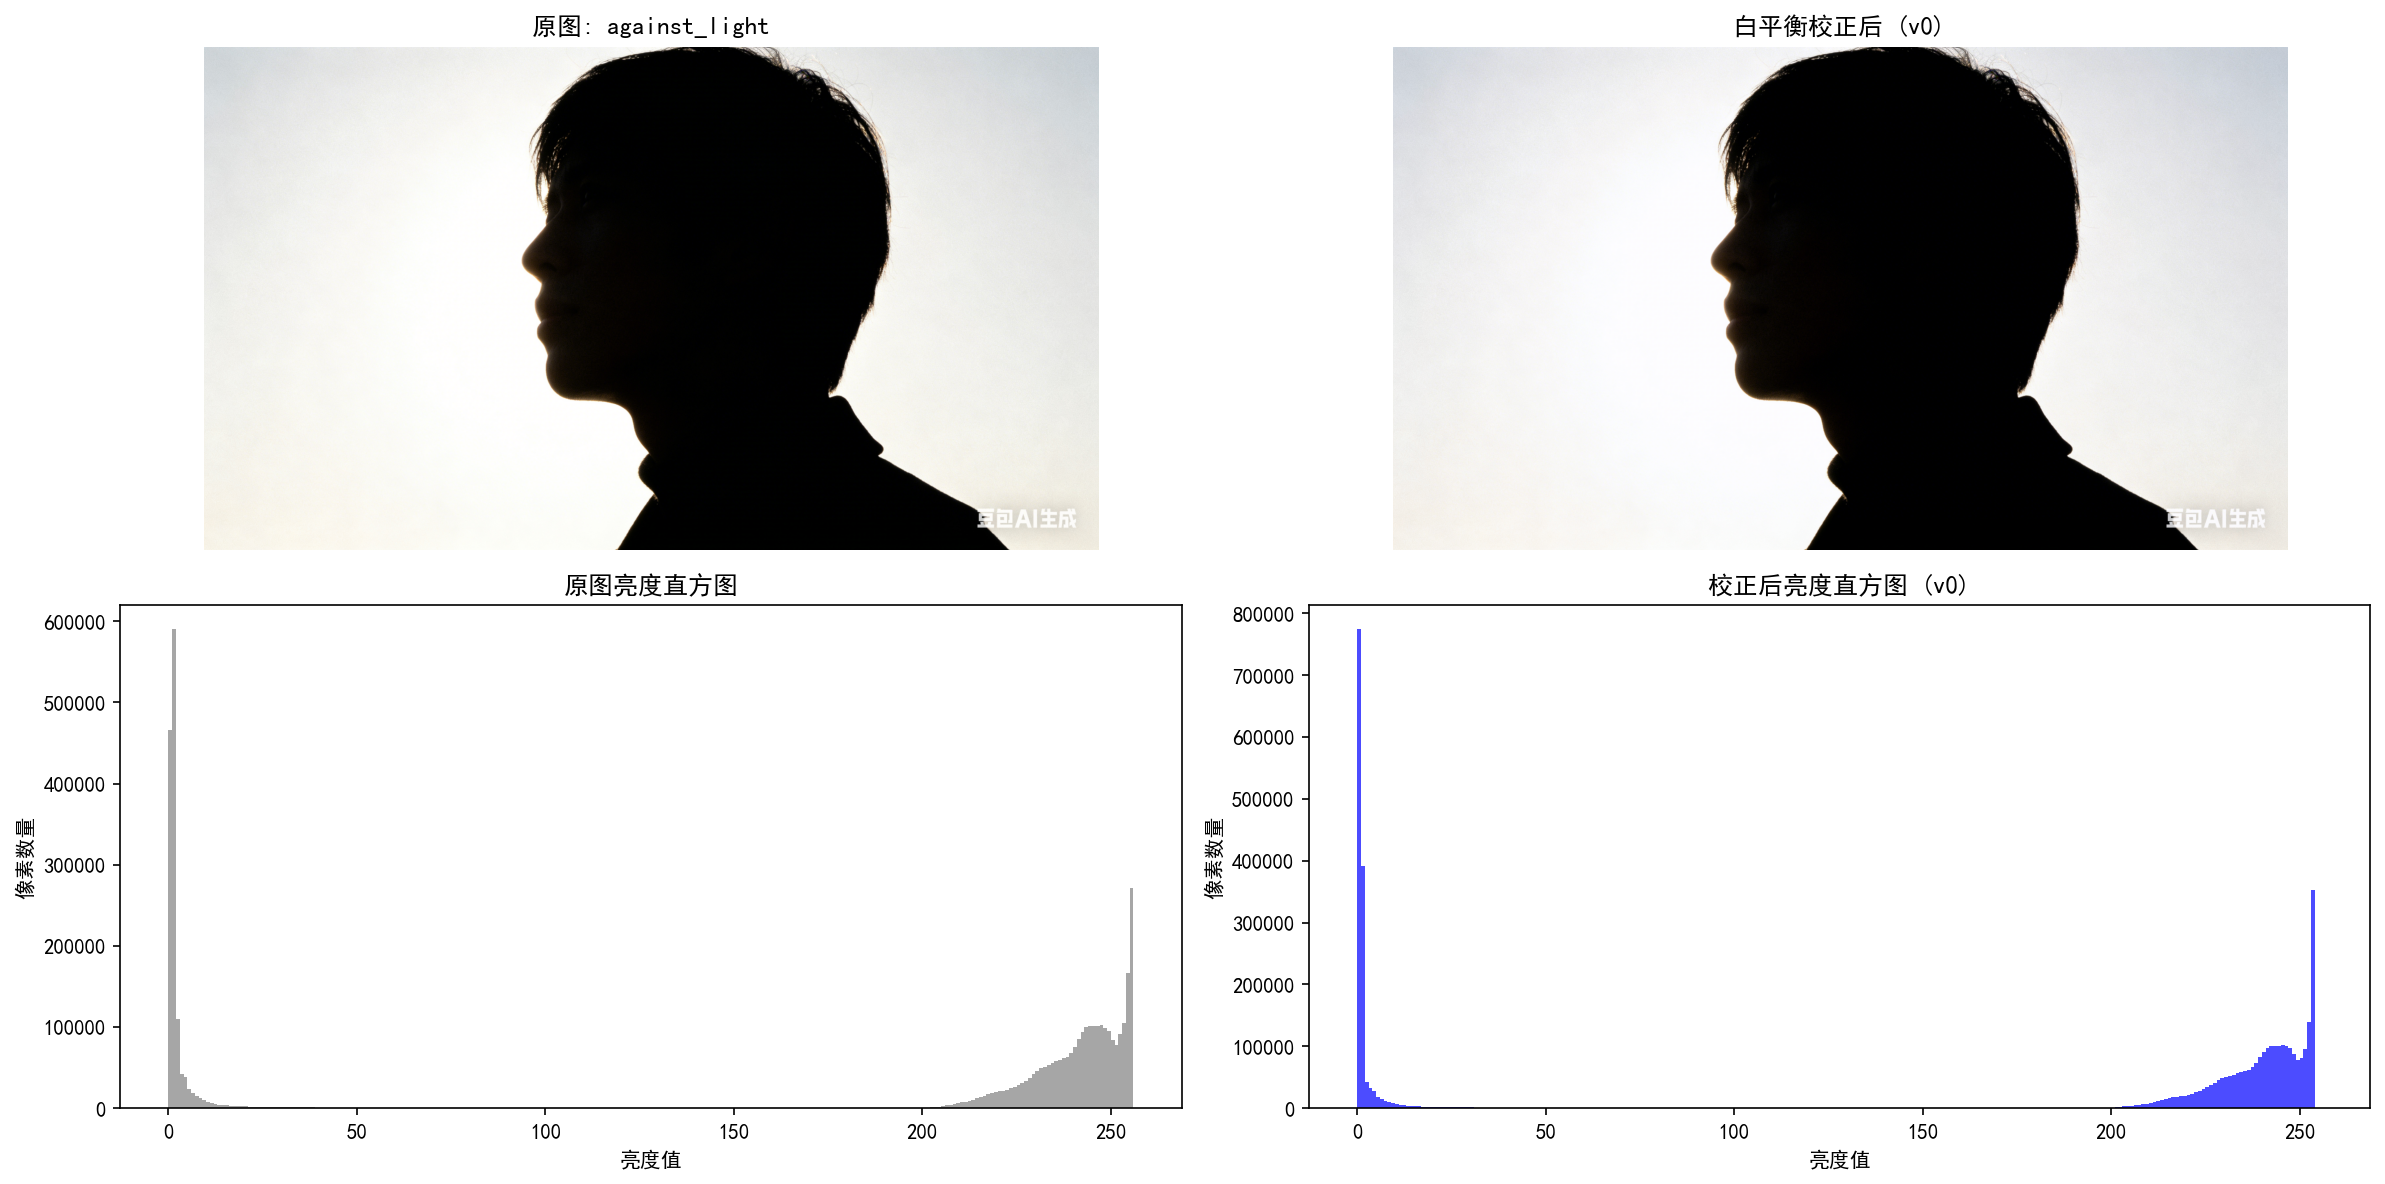
\includegraphics[width=\textwidth]{contrast/against_light_对比结果_v0.png}
        \caption{逆光人像：原版算法（v0）校正结果}
        \label{fig:against_v0}
    \end{minipage}
    \hfill
    \begin{minipage}{0.48\textwidth}
        \centering
        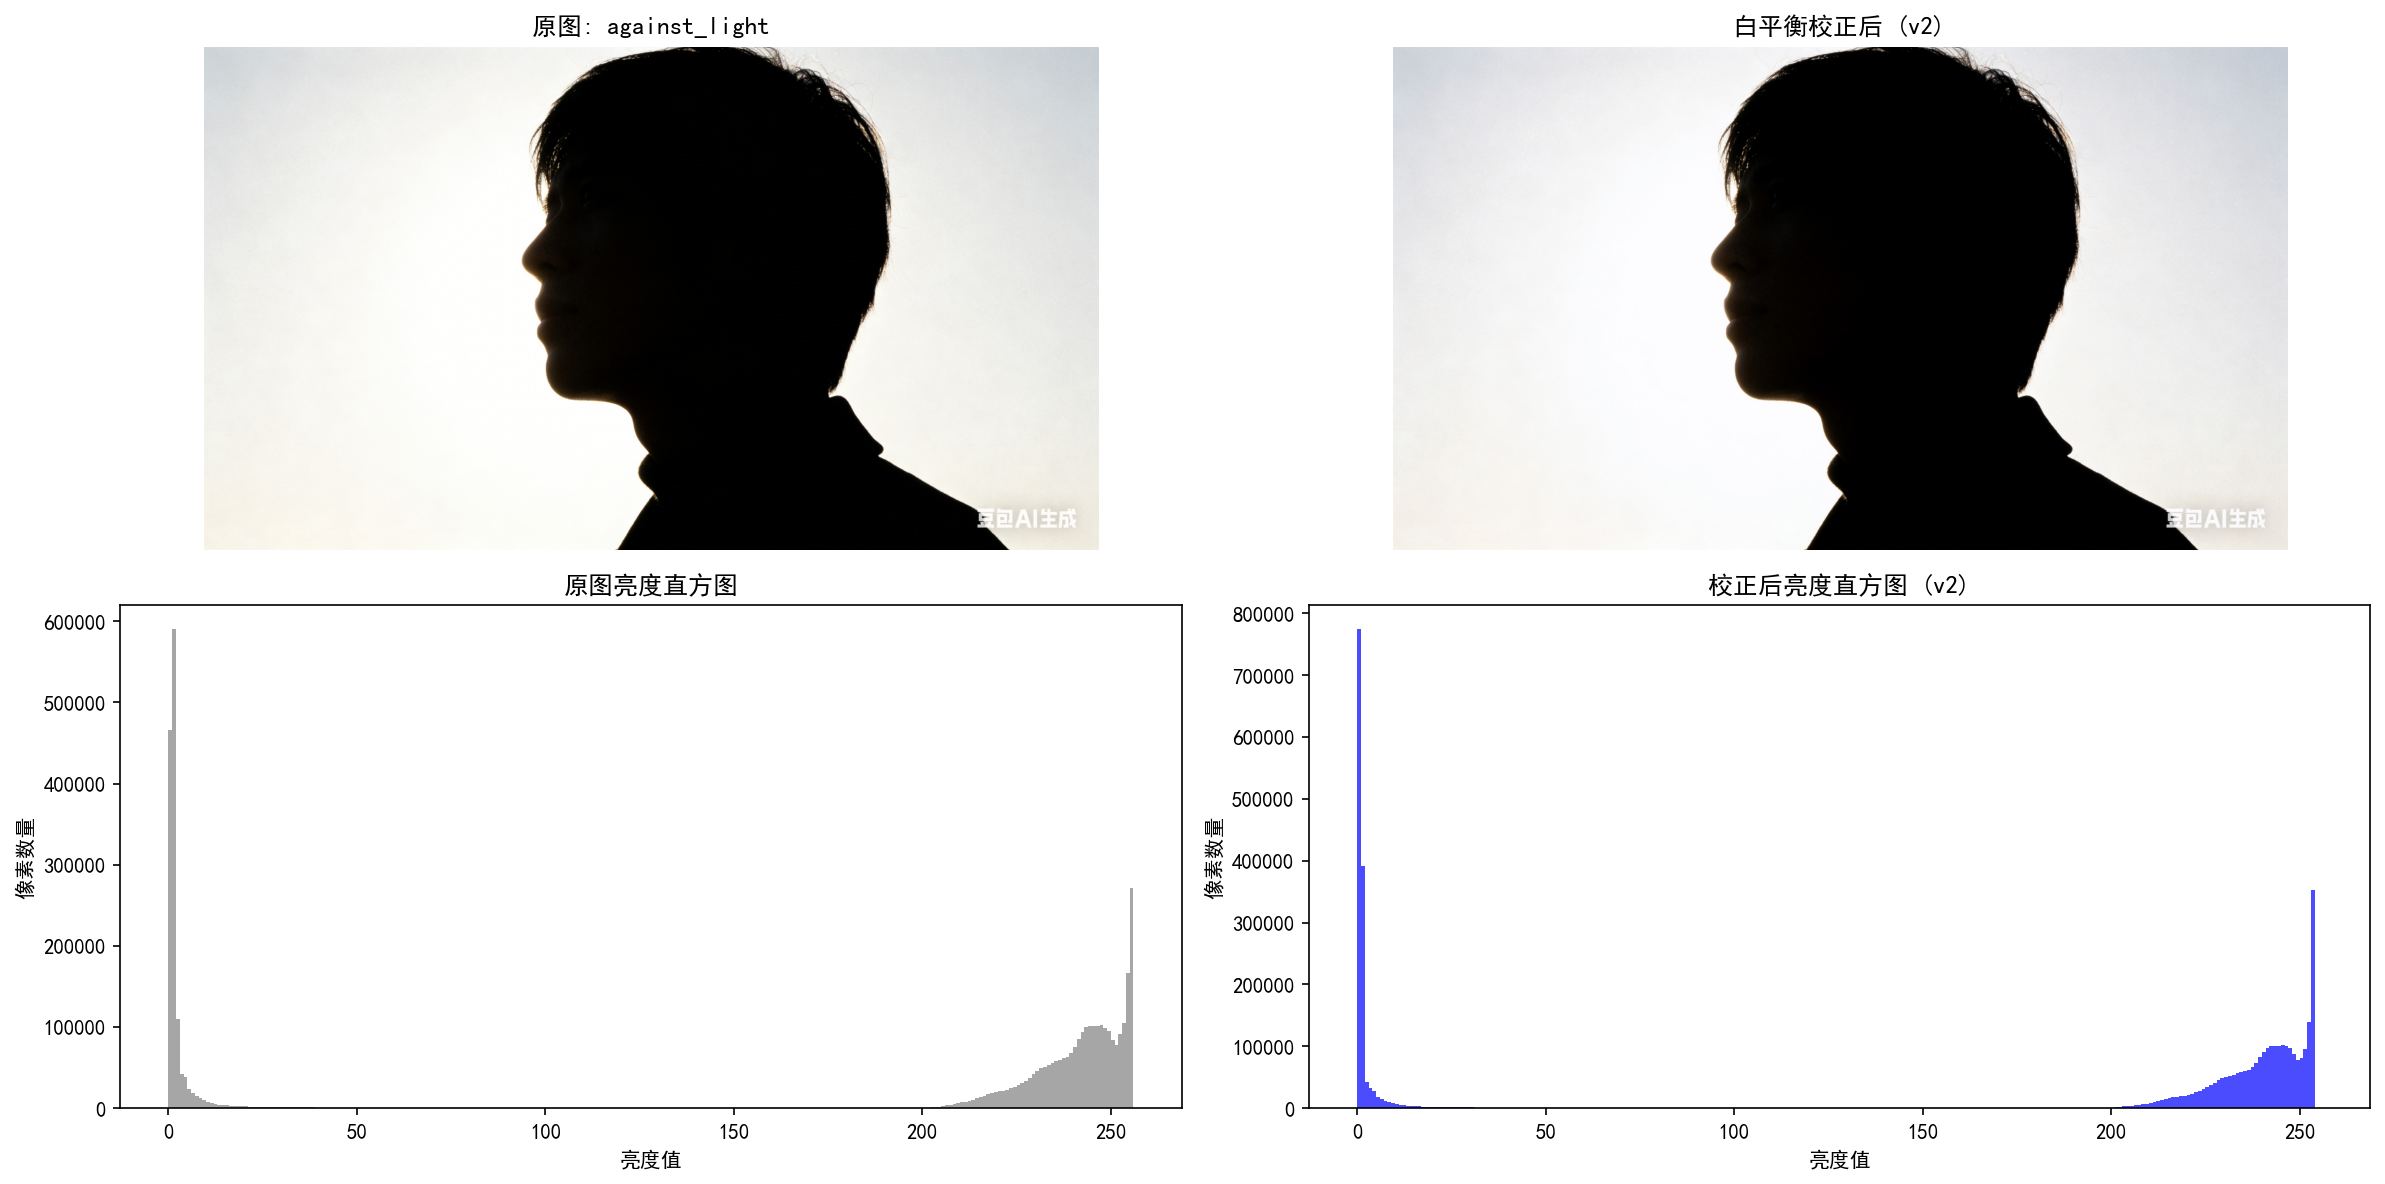
\includegraphics[width=\textwidth]{contrast/against_light_对比结果_v2.png}
        \caption{逆光人像：优化版算法（v2）校正结果（自动降级）}
        \label{fig:against_v2}
    \end{minipage}
\end{figure}

\begin{figure}[htbp]
    \centering
    \begin{minipage}{0.48\textwidth}
        \centering
        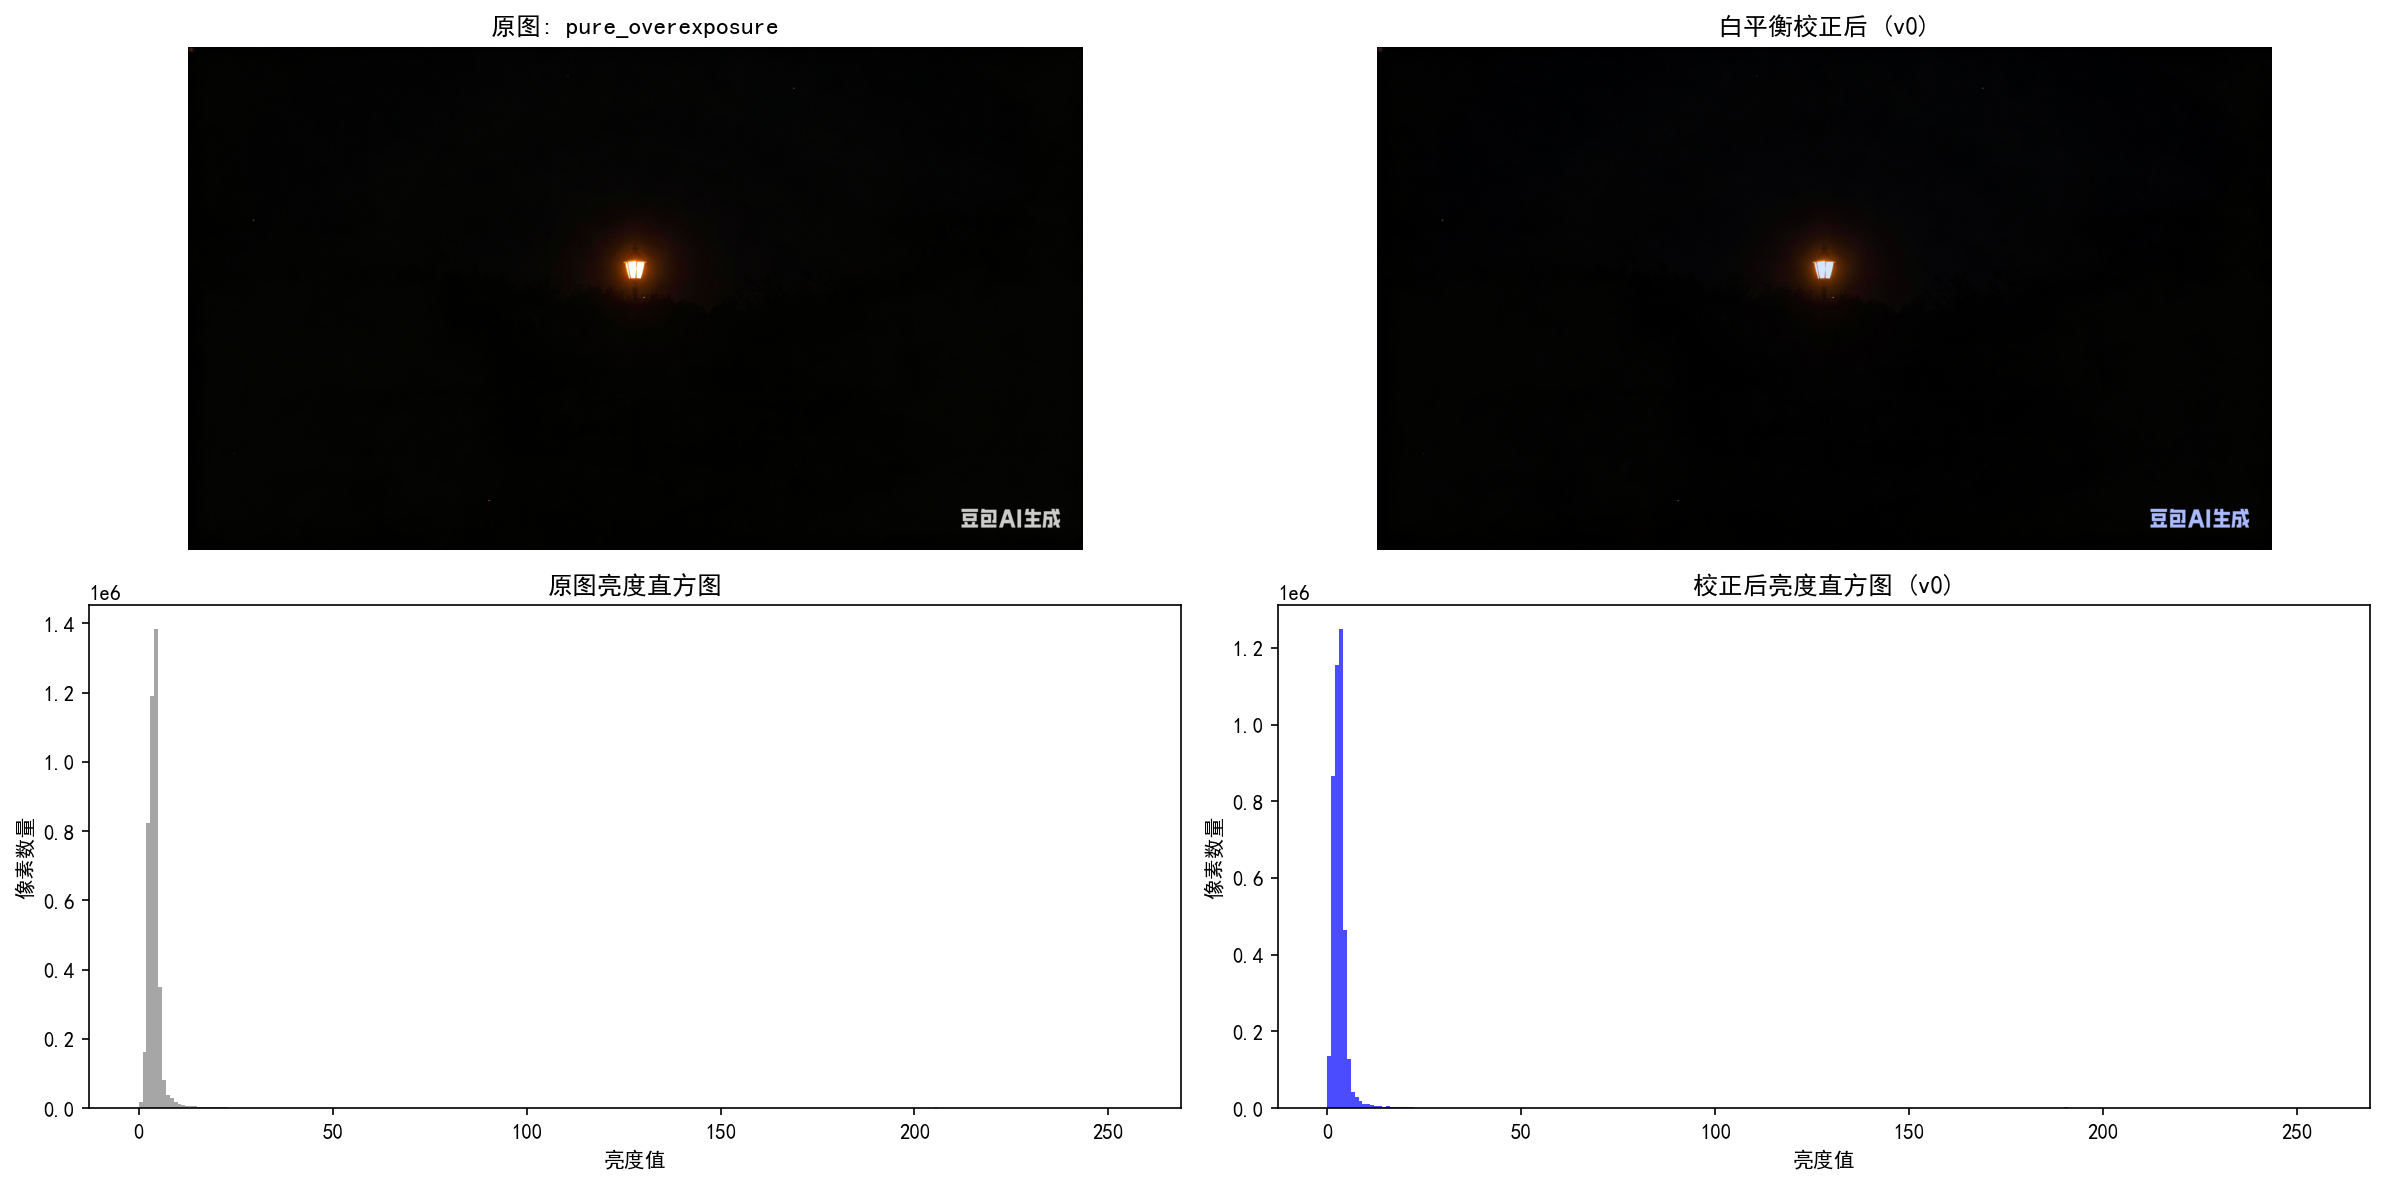
\includegraphics[width=\textwidth]{contrast/pure_overexposure_对比结果_v0.png}
        \caption{夜景路灯：原版算法（v0）校正结果}
        \label{fig:pure_v0}
    \end{minipage}
    \hfill
    \begin{minipage}{0.48\textwidth}
        \centering
        \includegraphics[width=\textwidth]{contrast/pure_overexposure_对比结果_v2.png}
        \caption{夜景路灯：优化版算法（v2）校正结果（自动降级）}
        \label{fig:pure_v2}
    \end{minipage}
\end{figure}

实验结果表明：优化版的自适应降级逻辑有效，在有效像素不足的极端场景下，不会引入额外的色彩失真，保证了算法的鲁棒性。

\subsection{场景二：算法局限性验证（大面积纯色场景）}
针对红色幕布这类“大面积单一色块”场景，灰度世界算法的核心假设不再成立，优化版算法的表现反而弱于原版，出现更严重的色彩失真。

\begin{figure}[htbp]
    \centering
    \begin{minipage}{0.48\textwidth}
        \centering
        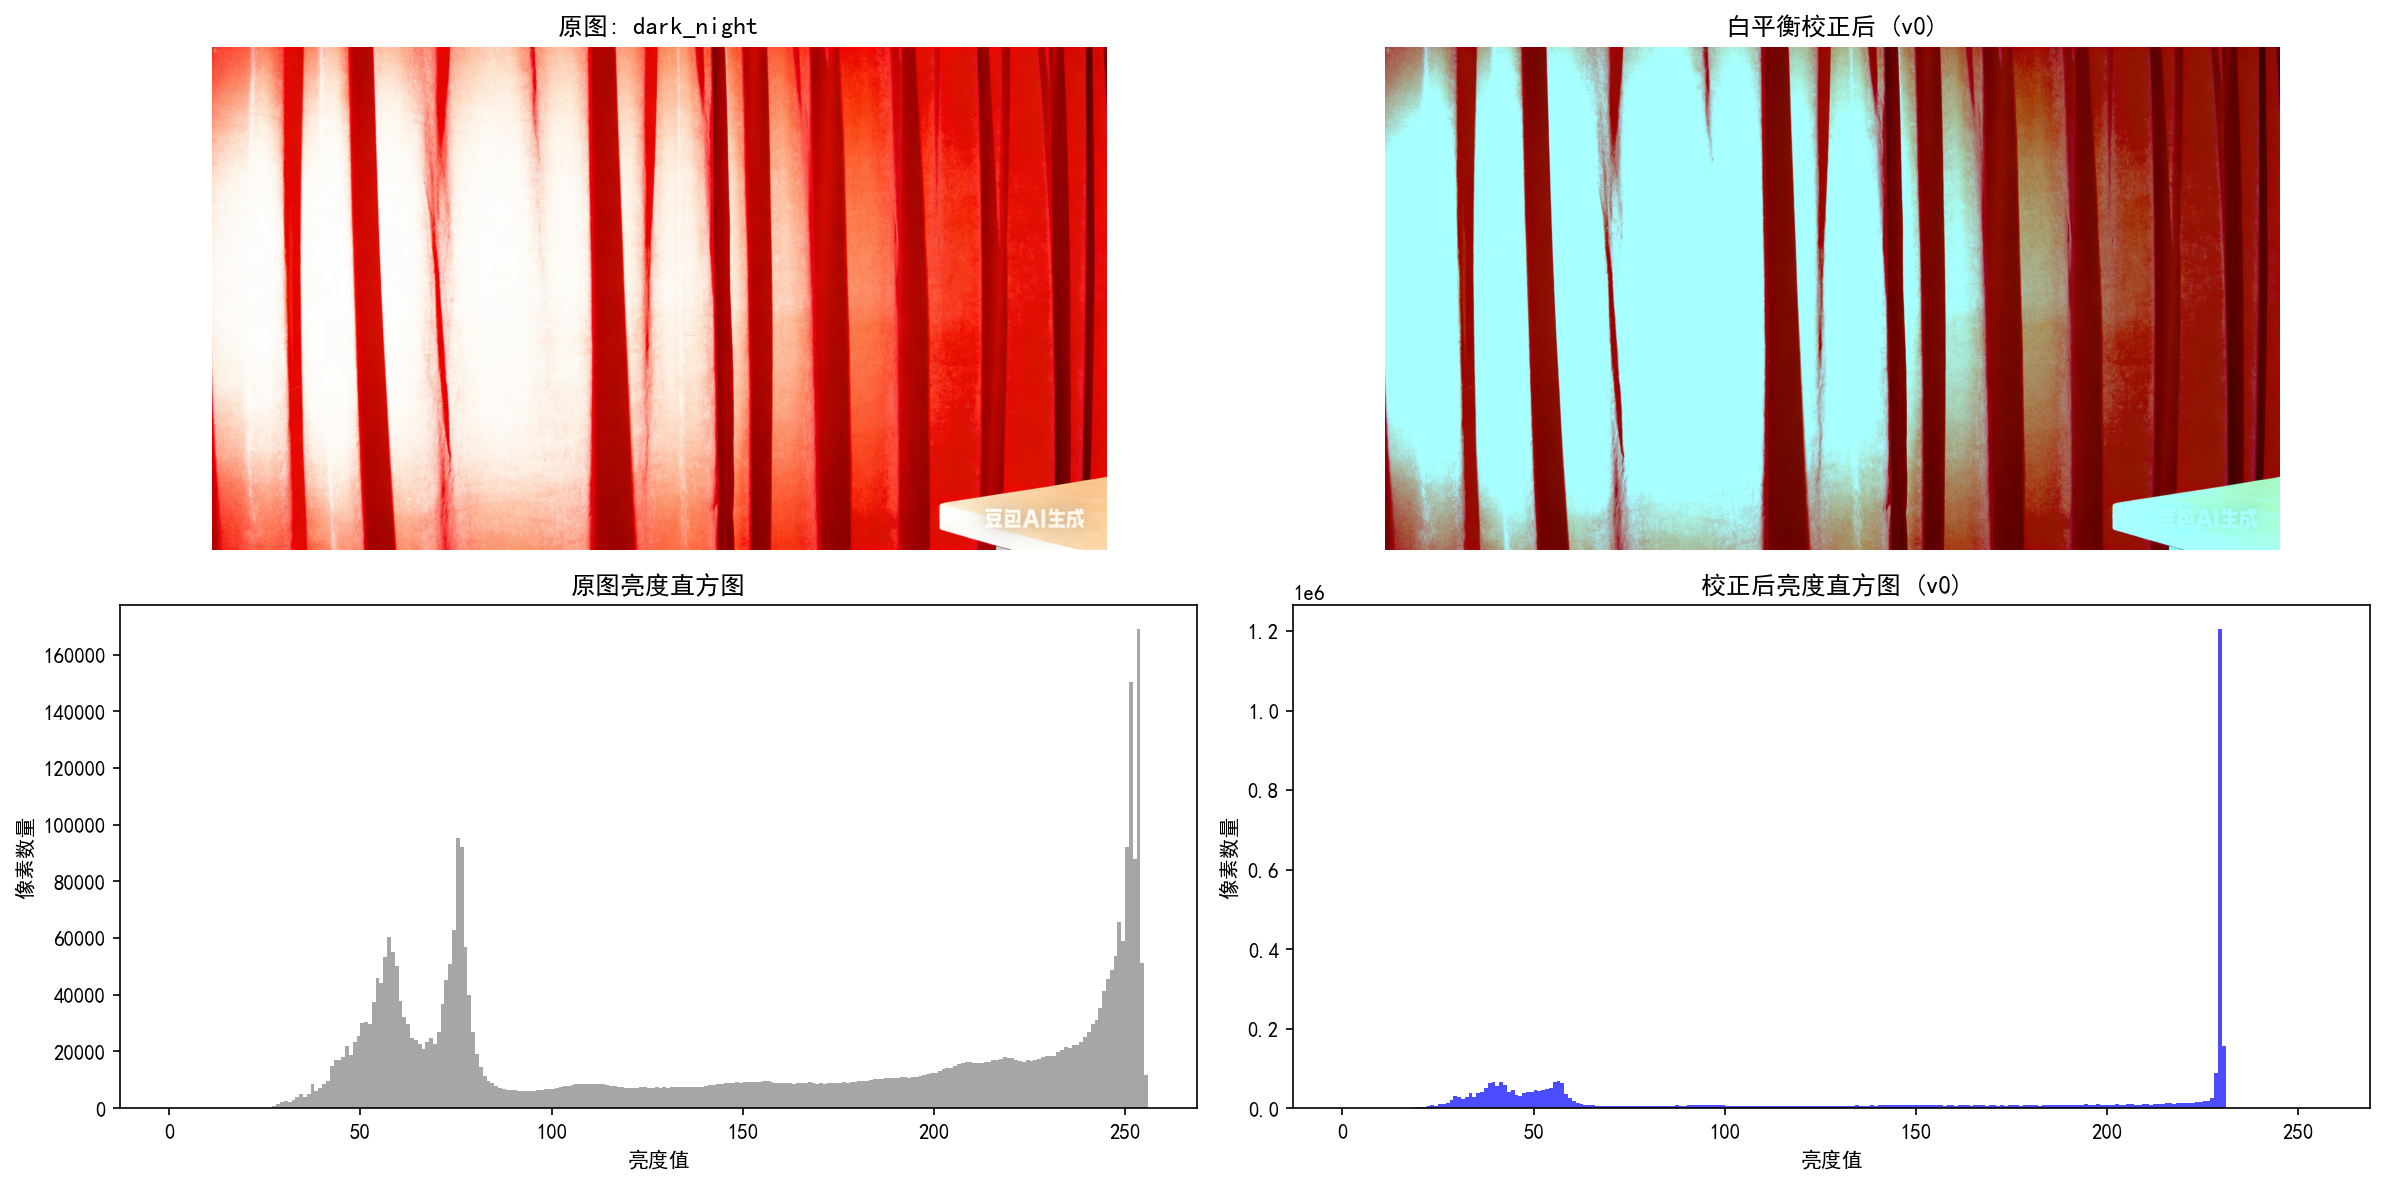
\includegraphics[width=\textwidth]{contrast/dark_night_对比结果_v0.png}
        \caption{红色幕布：原版算法（v0）校正结果}
        \label{fig:dark_v0}
    \end{minipage}
    \hfill
    \begin{minipage}{0.48\textwidth}
        \centering
        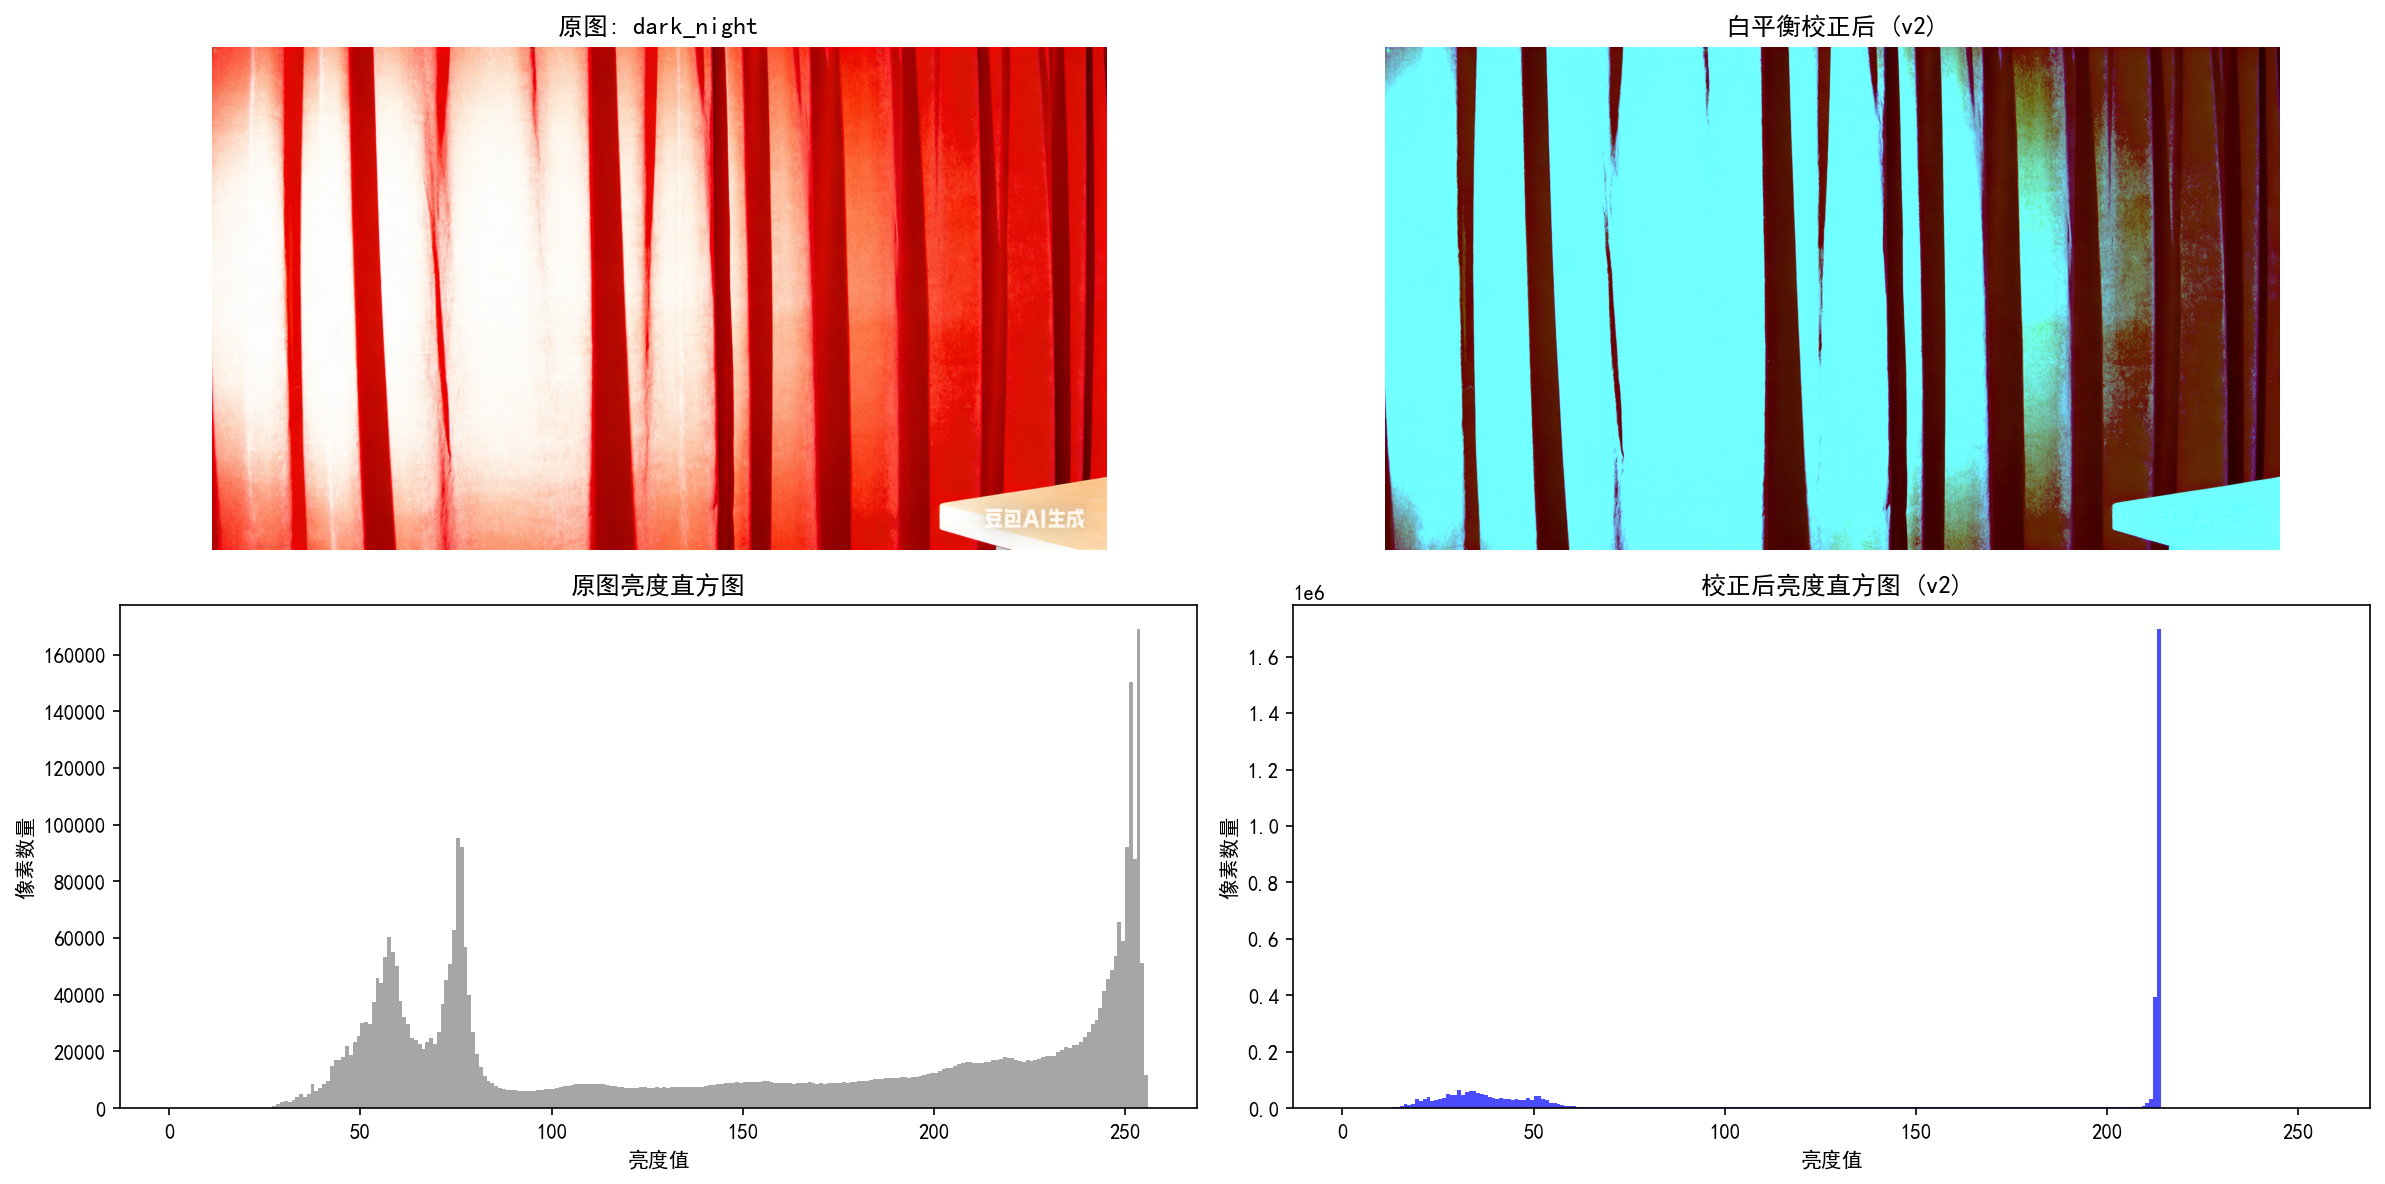
\includegraphics[width=\textwidth]{contrast/dark_night_对比结果_v2.png}
        \caption{红色幕布：优化版算法（v2）校正结果（色彩失真更严重）}
        \label{fig:dark_v2}
    \end{minipage}
\end{figure}

这一结果验证了灰度世界算法的固有局限性：当画面被单一颜色主导时，无论原版还是优化版算法，都无法实现准确的色彩还原；且优化版的像素筛选逻辑，会进一步压缩有效色彩信息，导致校正效果更差。

\subsection{场景三：常规色彩丰富场景验证}
针对色彩丰富的常规拍摄场景，优化版算法展现出了优秀的色彩还原能力，同时能较好地保留画面的氛围感。

\subsubsection{色彩鲜艳都市图}
对于色彩丰富、亮度均衡的都市图，原版与优化版的校正效果几乎无区别，算法稳定性良好，未出现过度校正问题。

\begin{figure}[htbp]
    \centering
    \includegraphics[width=0.8\textwidth]{contrast/色彩鲜艳_对比效果.jpg}
    \caption{色彩鲜艳都市图：原版与优化版校正效果几乎无差异}
    \label{fig:colorful}
\end{figure}

\subsubsection{怀旧小街图}
对于带有怀旧氛围感的街景图，优化版算法在校正偏色的同时，完整保留了画面的怀旧感、生活感与氛围感，色彩还原自然，未破坏画面的整体调性。

\begin{figure}[htbp]
    \centering
    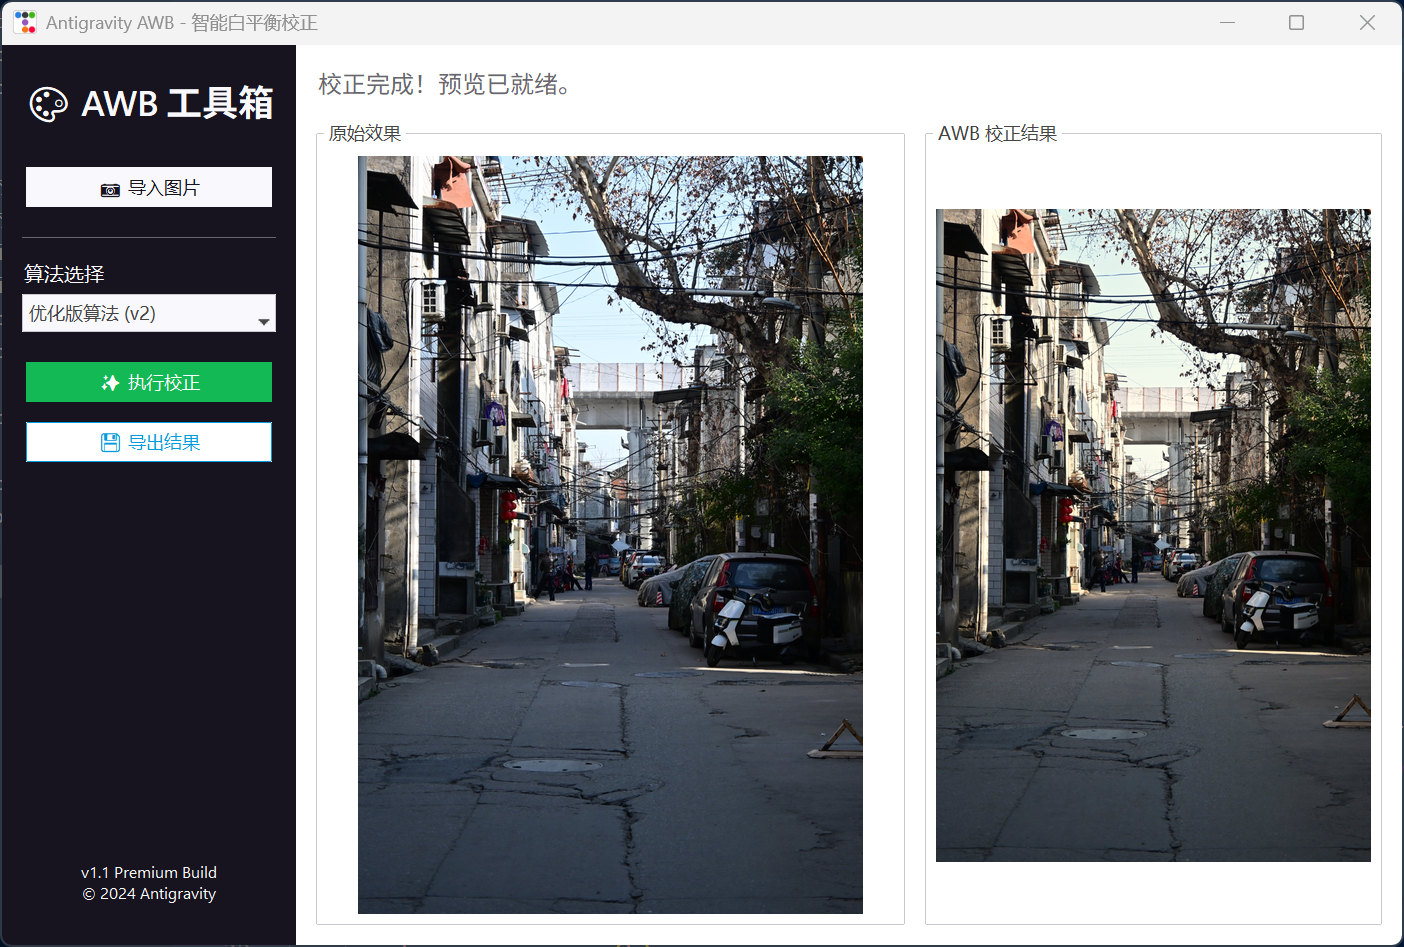
\includegraphics[width=0.8\textwidth]{contrast/小街_对比结果.jpg}
    \caption{怀旧小街图：优化版算法保留了画面的氛围感与生活感}
    \label{fig:street_old}
\end{figure}

\subsubsection{公园小路图}
对于公园小路图，优化版算法整体校正效果良好，但画面出现轻微偏紫的色彩偏差，仍存在一定的优化空间。

\begin{figure}[htbp]
    \centering
    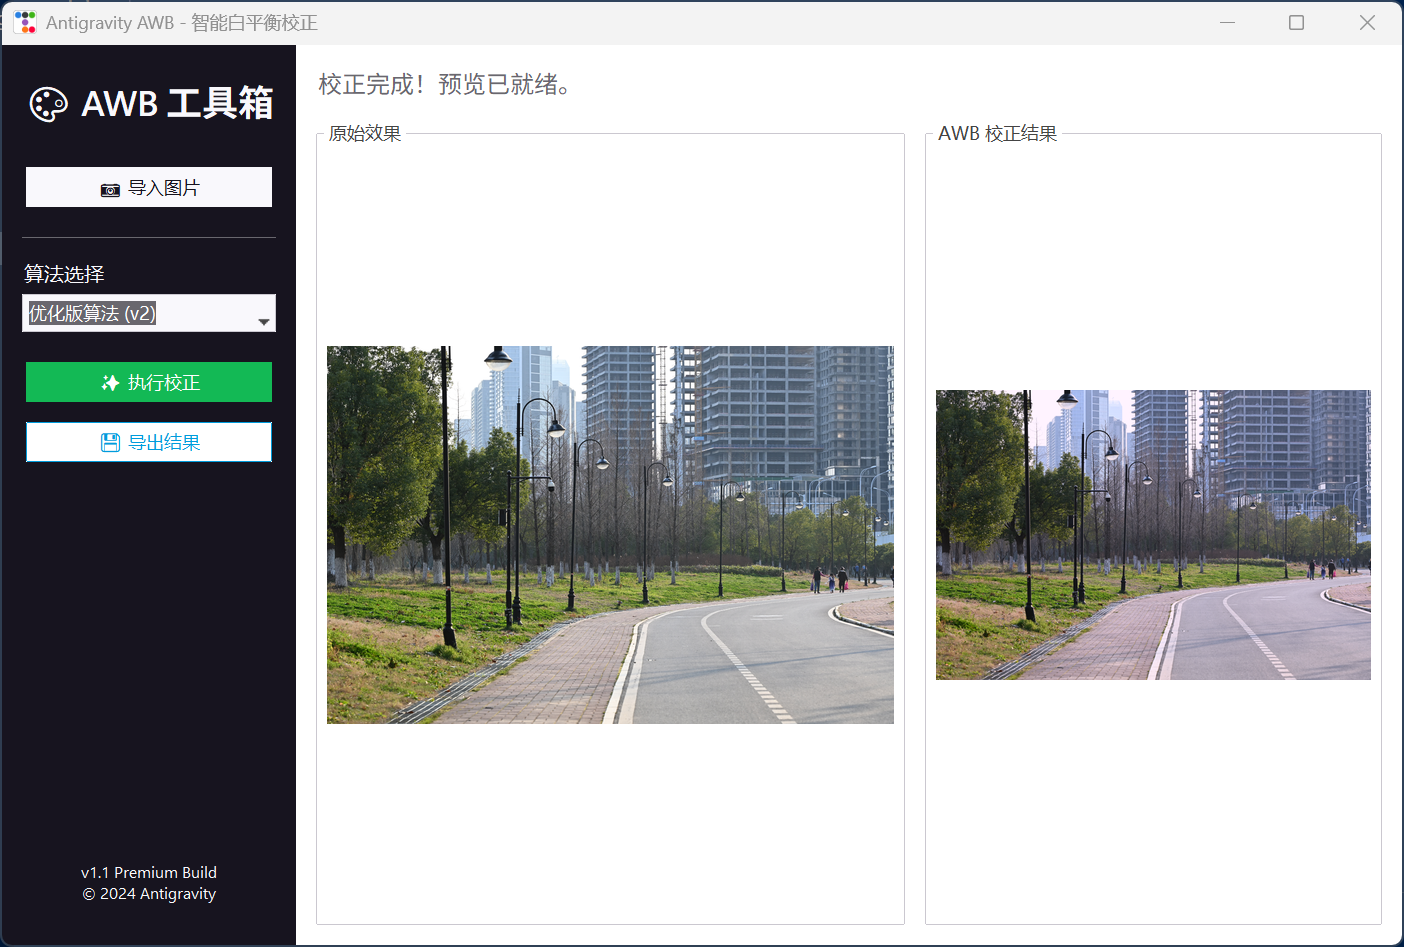
\includegraphics[width=0.8\textwidth]{contrast/街道_对比结果.jpg}
    \caption{公园小路图：优化版算法整体效果良好，存在轻微偏紫偏差}
    \label{fig:street_city}
\end{figure}

\begin{myresult}{实验核心结论}
    \begin{enumerate}
        \item \textbf{自适应性}：优化版算法的自适应降级逻辑有效，在极端低有效像素场景下，可避免过度校正，保证了算法的鲁棒性；
        \item \textbf{色彩表现}：色彩丰富的常规场景下，优化版算法色彩还原能力优秀，可较好保留画面氛围感，校正效果优于或持平原版算法；
        \item \textbf{固有限制}：大面积单一色块场景下，灰度世界算法的核心假设失效，原版与优化版均无法实现准确还原，这是经典算法的固有局限性；
        \item \textbf{优化空间}：部分复杂街景场景下，优化版算法仍存在轻微色彩偏差，后续可通过多算法融合进一步优化。
    \end{enumerate}
\end{myresult}

\section{GUI可视化界面展示}
为降低算法使用门槛，本项目基于 Ttkbootstrap 开发了现代化 GUI 界面，支持“导入-校正-导出”全流程可视化操作。已经在前面的图片中展示过
此处不再赘述。

\subsection{界面设计与功能模块}
GUI 界面采用“侧边栏+主显示区”布局，核心功能模块包括：
\begin{itemize}
    \item \textbf{图片导入模块}：支持 JPG/PNG/BMP 格式，兼容中文路径；
    \item \textbf{算法选择模块}：下拉框切换“基础版（v0）/优化版（v2）”算法；
    \item \textbf{校正执行模块}：一键运行算法，实时显示校正结果；
    \item \textbf{结果导出模块}：支持保存校正后图像为 JPG/PNG 格式；
    \item \textbf{可视化预览模块}：双栏对比显示原图与校正图，自适应缩放。
    \item \textbf{兼容性}：兼容 Windows/macOS/Linux 系统，支持中文路径。
\end{itemize}

\subsection{界面截图与操作流程}
\begin{figure}[htbp]
    \centering
    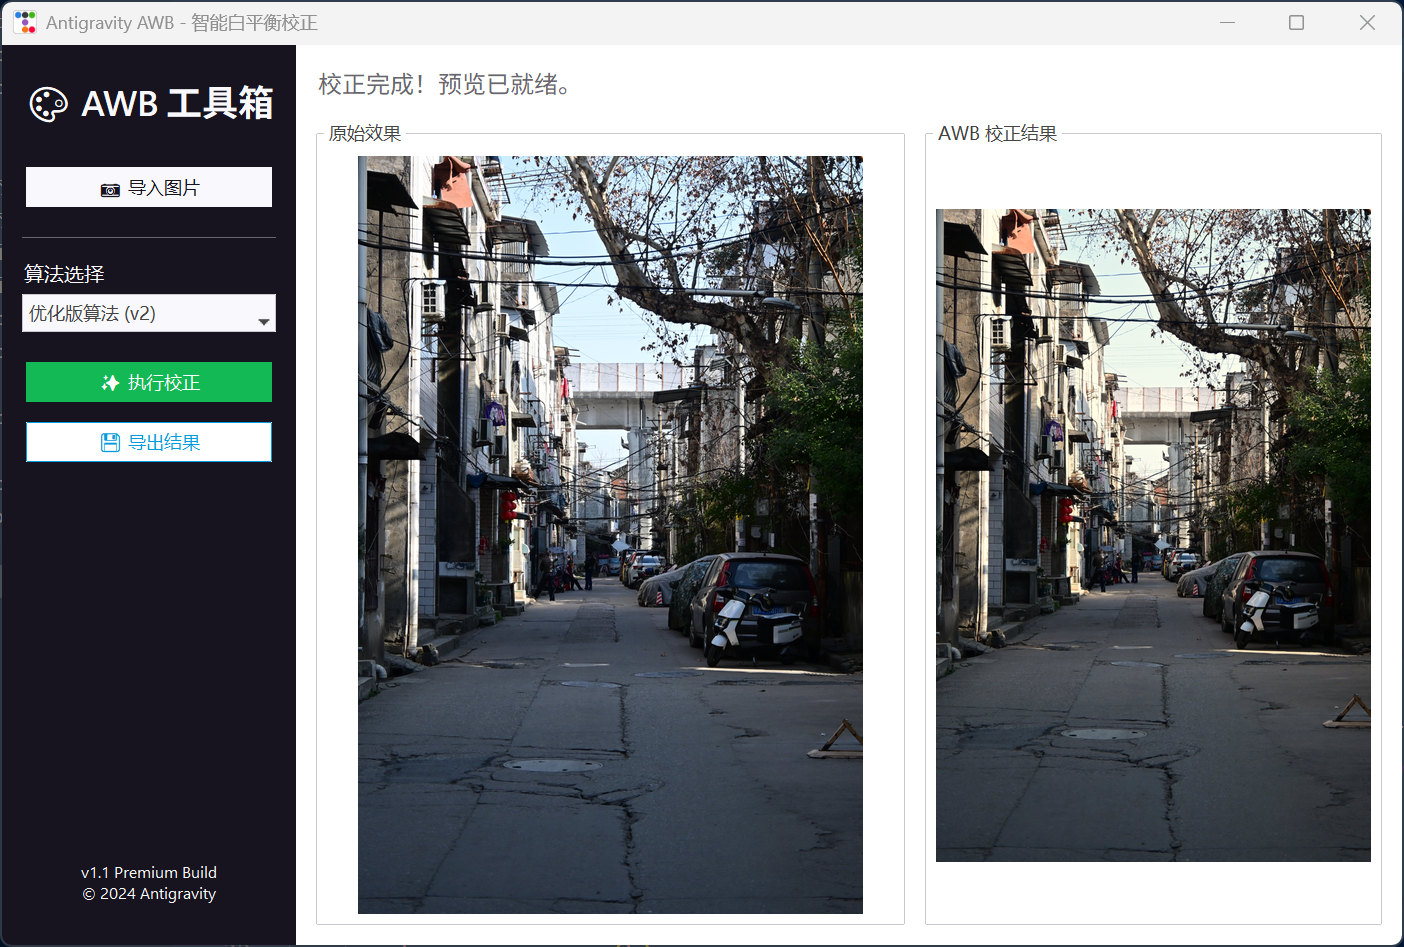
\includegraphics[width=0.9\textwidth]{contrast/小街_对比结果.jpg}
    \caption{AWB 智能白平衡校正工具 GUI 界面}
    \label{fig:gui_interface}
\end{figure}

操作流程（三步完成校正）：
\begin{enumerate}
    \item 点击「📷 导入图片」选择待校正图像；
    \item 在「算法选择」下拉框选择版本（推荐优化版），点击「✨ 执行校正」；
    \item 预览校正效果后，点击「💾 导出结果」保存图像。
\end{enumerate}

\subsection{GUI 核心优势}
\begin{itemize}
    \item \textbf{易用性}：无需编写代码，纯可视化操作；
    \item \textbf{交互性}：实时预览校正效果，支持多格式导出；
    \item \textbf{美观性}：采用现代化主题（Pulse），界面简洁易操作；
    \item \textbf{兼容性}：兼容 Windows/macOS/Linux 系统，支持中文路径。
\end{itemize}

\section{应用场景与后续规划}

本算法的落地将为多项实际任务奠定预处理基础：
\begin{itemize}
    \item \textbf{水利遥感}：统一不同时间段拍摄的河道图像色调，提升水位检测精度。
    \item \textbf{无人机巡检}：标准化航拍数据，消除光照剧烈变化对识别算法的影响。
\end{itemize}

下一步工作将集中于：
\begin{enumerate}
    \item 引入“完美反射算法”“色域映射算法”，构建多算法融合的 AWB 工具；
    \item 优化 GUI 功能，增加批量处理、直方图可视化、色温手动调节模块；
    \item 针对水利/无人机场景的图像特征，定制化优化算法参数，提升场景适配性。
\end{enumerate}

% ======================================================
% 附录：完整Demo代码
% ======================================================
\newpage
\section*{附录：完整Demo代码}
\addcontentsline{toc}{section}{附录：完整Demo代码}

\begin{lstlisting}[caption={完整的自动白平衡Demo代码（awb\_demo_v2.py）}, label=code:full]
import cv2
import numpy as np
import matplotlib.pyplot as plt
import os

# ========== 解决matplotlib中文乱码 ==========
plt.rcParams['font.sans-serif'] = ['SimHei']
plt.rcParams['axes.unicode_minus'] = False

# ========== 适配文件夹结构（固定相对路径）==========
ORIGINAL_FOLDER = "original"
OPTIMIZED_FOLDER = "optimized"
CONTRAST_FOLDER = "contrast"

os.makedirs(ORIGINAL_FOLDER, exist_ok=True)
os.makedirs(OPTIMIZED_FOLDER, exist_ok=True)
os.makedirs(CONTRAST_FOLDER, exist_ok=True)
# =================================================

# ===================== 1. 核心算法（双版本：原版+优化版）=====================
def gray_world_awb(image_path, use_optimized=False):
    try:
        img = cv2.imdecode(np.fromfile(image_path, dtype=np.uint8), cv2.IMREAD_COLOR)
    except Exception as e:
        print(f"❌ 读取图片出错: {image_path}, 错误: {e}")
        return None, None
    
    if img is None:
        print(f"❌ 无法读取图片: {image_path}")
        return None, None
    
    b, g, r = cv2.split(img)
    
    if use_optimized:
        gray = cv2.cvtColor(img, cv2.COLOR_BGR2GRAY)
        mask = (gray >= 60) & (gray <= 180)
        valid_ratio = np.sum(mask)/mask.size
        if valid_ratio >= 0.1:
            b_avg = np.mean(b[mask])
            g_avg = np.mean(g[mask])
            r_avg = np.mean(r[mask])
            print(f"   ✨ 使用优化版算法（中亮度像素占比: {valid_ratio:.1%}）")
        else:
            b_avg = np.mean(b)
            g_avg = np.mean(g)
            r_avg = np.mean(r)
            print(f"   ⚠️ 中亮度像素占比不足{valid_ratio:.1%}，自动切换为原版算法")
    else:
        b_avg = np.mean(b)
        g_avg = np.mean(g)
        r_avg = np.mean(r)
        print(f"   📌 使用原版算法（全局像素均值）")
    
    K = (b_avg + g_avg + r_avg) / 3.0
    gain_b = K / (b_avg + 1e-6)
    gain_g = K / (g_avg + 1e-6)
    gain_r = K / (r_avg + 1e-6)
    
    b_new = np.clip(b.astype(float) * gain_b, 0, 255)
    g_new = np.clip(g.astype(float) * gain_g, 0, 255)
    r_new = np.clip(r.astype(float) * gain_r, 0, 255)
    
    img_awb = cv2.merge([b_new.astype(np.uint8), 
                          g_new.astype(np.uint8), 
                          r_new.astype(np.uint8)])
    return img, img_awb

# ===================== 2. 可视化对比 =====================
def show_comparison(original_img, awb_img, img_name, version_suffix):
    original_rgb = cv2.cvtColor(original_img, cv2.COLOR_BGR2RGB)
    awb_rgb = cv2.cvtColor(awb_img, cv2.COLOR_BGR2RGB)
    original_gray = cv2.cvtColor(original_img, cv2.COLOR_BGR2GRAY)
    awb_gray = cv2.cvtColor(awb_img, cv2.COLOR_BGR2GRAY)
    
    plt.figure(figsize=(16, 8))
    
    plt.subplot(2, 2, 1)
    plt.imshow(original_rgb)
    plt.title(f'原图: {img_name}')
    plt.axis('off')
    
    plt.subplot(2, 2, 2)
    plt.imshow(awb_rgb)
    plt.title(f'白平衡校正后 ({version_suffix})')
    plt.axis('off')
    
    plt.subplot(2, 2, 3)
    plt.hist(original_gray.ravel(), bins=256, range=[0, 256], color='gray', alpha=0.7)
    plt.title('原图亮度直方图')
    plt.xlabel('亮度值')
    plt.ylabel('像素数量')
    
    plt.subplot(2, 2, 4)
    plt.hist(awb_gray.ravel(), bins=256, range=[0, 256], color='blue', alpha=0.7)
    plt.title(f'校正后亮度直方图 ({version_suffix})')
    plt.xlabel('亮度值')
    plt.ylabel('像素数量')
    
    save_path = os.path.join(CONTRAST_FOLDER, f'{img_name}_对比结果_{version_suffix}.png')
    plt.tight_layout()
    plt.savefig(save_path, dpi=150, bbox_inches='tight')
    plt.close()
    print(f"   💾 对比图已保存: {save_path}")

# ===================== 3. 批量处理 =====================
def process_single_version(use_optimized, version_suffix):
    supported_ext = ('.jpg', '.jpeg', '.png', '.bmp', '.JPG', '.JPEG', '.PNG')
    
    print(f"\n{'='*60}")
    print(f"🚀 开始处理【{version_suffix}】版本...")
    print(f"{'='*60}")
    
    img_count = 0
    for filename in os.listdir(ORIGINAL_FOLDER):
        if filename.endswith(supported_ext):
            img_count += 1
            img_path = os.path.join(ORIGINAL_FOLDER, filename)
            img_name = os.path.splitext(filename)[0]
            
            print(f"\n[{img_count}] 处理图片: {filename}")
            
            original, awb_result = gray_world_awb(img_path, use_optimized=use_optimized)
            if original is None or awb_result is None:
                continue
            
            show_comparison(original, awb_result, img_name, version_suffix)
            
            save_img_path = os.path.join(OPTIMIZED_FOLDER, f'{img_name}_校正后_{version_suffix}.jpg')
            _, img_encode = cv2.imencode('.jpg', awb_result)
            img_encode.tofile(save_img_path)
            print(f"   💾 校正图已保存: {save_img_path}")
    
    print(f"\n{'='*60}")
    if img_count == 0:
        print(f"❌ 【{version_suffix}】版本处理失败：original文件夹里没有找到图片！")
    else:
        print(f"✅ 【{version_suffix}】版本处理完成！共处理 {img_count} 张图片")
    print(f"{'='*60}\n")

# ===================== 4. 主函数 =====================
if __name__ == "__main__":
    RUN_V0 = True
    RUN_V2 = True
    
    print("\n" + "="*60)
    print("📋 运行配置：")
    if RUN_V0:
        print("   ✅ 运行【原版算法】（v0）")
    if RUN_V2:
        print("   ✅ 运行【优化版算法】（v2）")
    print("="*60)
    
    if RUN_V0:
        process_single_version(use_optimized=False, version_suffix="v0")
    
    if RUN_V2:
        process_single_version(use_optimized=True, version_suffix="v2")
    
    print("\n🎉 所有任务已完成！")
    print(f"   校正后图片在：{os.path.abspath(OPTIMIZED_FOLDER)}")
    print(f"   对比结果在：{os.path.abspath(CONTRAST_FOLDER)}")
\end{lstlisting}

\begin{lstlisting}[caption={AWB可视化GUI代码（awb\_gui.py）}, label=code:gui]
import cv2
import numpy as np
import tkinter as tk
from tkinter import filedialog, messagebox
from PIL import Image, ImageTk
import ttkbootstrap as ttk
from ttkbootstrap.constants import *
from ttkbootstrap.widgets import ToastNotification

# ========== 1. 核心算法 ==========
def gray_world_awb(img, use_optimized=False):
    b, g, r = cv2.split(img)
    
    if use_optimized:
        gray = cv2.cvtColor(img, cv2.COLOR_BGR2GRAY)
        mask = (gray >= 60) & (gray <= 180)
        valid_ratio = np.sum(mask)/mask.size
        if valid_ratio >= 0.1:
            b_avg = np.mean(b[mask])
            g_avg = np.mean(g[mask])
            r_avg = np.mean(r[mask])
        else:
            b_avg = np.mean(b)
            g_avg = np.mean(g)
            r_avg = np.mean(r)
    else:
        b_avg = np.mean(b)
        g_avg = np.mean(g)
        r_avg = np.mean(r)
    
    K = (b_avg + g_avg + r_avg) / 3.0
    gain_b = K / (b_avg + 1e-6)
    gain_g = K / (g_avg + 1e-6)
    gain_r = K / (r_avg + 1e-6)
    
    b_new = np.clip(b.astype(float) * gain_b, 0, 255)
    g_new = np.clip(g.astype(float) * gain_g, 0, 255)
    r_new = np.clip(r.astype(float) * gain_r, 0, 255)
    
    return cv2.merge([b_new.astype(np.uint8), g_new.astype(np.uint8), r_new.astype(np.uint8)])

# ========== 2. GUI 设计 ==========
class AWBApp:
    def __init__(self, root):
        self.root = root
        self.root.title("Antigravity AWB - 智能白平衡校正")
        self.root.geometry("1400x900")
        
        self.original_img = None
        self.processed_img = None
        self.current_path = None
        
        self.setup_ui()

    def setup_ui(self):
        # 侧边栏
        self.sidebar = ttk.Frame(self.root, bootstyle=DARK, width=300, padding=20)
        self.sidebar.pack(side=LEFT, fill=Y)
        
        ttk.Label(self.sidebar, text="🎨 AWB 工具箱", font=("Segoe UI Variable Display Semibold", 18), 
                  bootstyle=(INVERSE, DARK)).pack(pady=(10, 30))
        
        controls_frame = ttk.Frame(self.sidebar, bootstyle=DARK)
        controls_frame.pack(fill=X)
        
        self.btn_open = ttk.Button(controls_frame, text="📷 导入图片", command=self.open_image, 
                                   bootstyle=LIGHT, width=20)
        self.btn_open.pack(pady=10)
        
        ttk.Separator(controls_frame, bootstyle=SECONDARY).pack(fill=X, pady=20)
        
        ttk.Label(controls_frame, text="算法选择", font=("微软雅黑", 10), bootstyle=(INVERSE, DARK)).pack(anchor=W)
        self.algo_var = tk.StringVar(value="优化版算法 (v2)")
        self.algo_combo = ttk.Combobox(controls_frame, textvariable=self.algo_var, 
                                       values=["基础版算法 (v0)", "优化版算法 (v2)"],
                                       state="readonly")
        self.algo_combo.pack(fill=X, pady=(5, 20))
        
        self.btn_process = ttk.Button(controls_frame, text="✨ 执行校正", command=self.process_image, 
                                      bootstyle=SUCCESS, width=20)
        self.btn_process.pack(pady=10)
        
        self.btn_save = ttk.Button(controls_frame, text="💾 导出结果", command=self.save_image, 
                                   bootstyle=(INFO, OUTLINE), width=20)
        self.btn_save.pack(pady=10)
        
        ttk.Label(self.sidebar, text="v1.1 Premium Build\n© 2026 Antigravity", 
                  font=("Segoe UI", 8), bootstyle=(INVERSE, DARK), justify=CENTER).pack(side=BOTTOM, pady=20)
        
        # 主显示区
        self.main_content = ttk.Frame(self.root, padding=20)
        self.main_content.pack(side=LEFT, fill=BOTH, expand=True)
        
        self.header_frame = ttk.Frame(self.main_content)
        self.header_frame.pack(fill=X, pady=(0, 20))
        self.status_var = tk.StringVar(value="等待导入...")
        ttk.Label(self.header_frame, textvariable=self.status_var, font=("Segoe UI", 12), 
                  bootstyle=SECONDARY).pack(side=LEFT)
        
        self.view_port = ttk.Frame(self.main_content)
        self.view_port.pack(fill=BOTH, expand=True)
        
        self.left_card = ttk.Labelframe(self.view_port, text=" 原始效果 ", padding=10)
        self.left_card.pack(side=LEFT, fill=BOTH, expand=True, padx=(0, 10))
        self.canvas_left = tk.Canvas(self.left_card, bg="#f8f9fa", highlightthickness=0)
        self.canvas_left.pack(fill=BOTH, expand=True)
        
        self.right_card = ttk.Labelframe(self.view_port, text=" AWB 校正结果 ", padding=10)
        self.right_card.pack(side=LEFT, fill=BOTH, expand=True, padx=(10, 0))
        self.canvas_right = tk.Canvas(self.right_card, bg="#f8f9fa", highlightthickness=0)
        self.canvas_right.pack(fill=BOTH, expand=True)

    def open_image(self):
        file_path = filedialog.askopenfilename(filetypes=[("Image Files", "*.jpg *.jpeg *.png *.bmp")])
        if not file_path:
            return
            
        self.current_path = file_path
        self.original_img = cv2.imread(file_path)
        self.show_on_canvas(self.original_img, self.canvas_left)
        self.status_var.set(f"已加载: {file_path.split('/')[-1]}")
        
        self.canvas_right.delete("all")
        self.processed_img = None

    def process_image(self):
        if self.original_img is None:
            ToastNotification(title="提示", message="请先导入一张图片", duration=3000, bootstyle=WARNING).show()
            return
            
        use_optimized = "优化版" in self.algo_var.get()
        self.processed_img = gray_world_awb(self.original_img, use_optimized=use_optimized)
        self.show_on_canvas(self.processed_img, self.canvas_right)
        self.status_var.set("校正完成！预览已就绪。")
        ToastNotification(title="成功", message="智能白平衡算法处理完毕", duration=2000, bootstyle=SUCCESS).show_toast()

    def save_image(self):
        if self.processed_img is None:
            messagebox.showwarning("警告", "没有可供保存的校正结果！")
            return
            
        path = filedialog.asksaveasfilename(defaultextension=".jpg", 
                                            filetypes=[("JPG Image", "*.jpg"), ("PNG Image", "*.png")])
        if path:
            cv2.imwrite(path, self.processed_img)
            ToastNotification(title="导出成功", message=f"图片已保存至该位置", duration=3000, bootstyle=INFO).show_toast()

    def show_on_canvas(self, img, canvas):
        img_rgb = cv2.cvtColor(img, cv2.COLOR_BGR2RGB)
        img_pil = Image.fromarray(img_rgb)
        
        self.root.update_idletasks()
        cw = canvas.winfo_width()
        ch = canvas.winfo_height()
        
        if cw < 10: cw, ch = 600, 600
        
        img_pil.thumbnail((cw, ch), Image.Resampling.LANCZOS)
        img_tk = ImageTk.PhotoImage(img_pil)
        
        canvas.delete("all")
        canvas.create_image(cw//2, ch//2, anchor=CENTER, image=img_tk)
        canvas.image = img_tk

if __name__ == "__main__":
    root = ttk.Window(themename="pulse")
    app = AWBApp(root)
    root.mainloop()
\end{lstlisting}

\end{document}